A couple of neutral atoms interacting through Lennard-Jones potentials hardly 
feel each other as soon as they separate farther than three or four times 
$\sigma$, even if one of them is just the nearest of a huge cluster of atoms. 
Long-range interactions fall off much more slowly. The Earth feels the tug of 
the sun bending its trajectory from many millions of miles away. In the latter 
case, we cannot define a cut-off radius for interactions. In classical physics, 
the Earth will feel the attraction of other heavenly bodies no matter the 
distance, as huge masses compensate for greater separations.

\section{Gravity}

You probably know that Newtonian gravitational forces obey an inverse-square
law, with the force of object $i$ on object $j$ given by
\begin{equation*}
  F(\mathrm{r}_{ij}) = -G \frac{m_i m_j}{r_{ij}^2}\
                          \frac{\mathbf{r}_{ij}}{r_{ij}},
\end{equation*}
with $\mathbf{r}_{ij}$ standing for the vector going from $i$ to $j$, $m_i$ and
$m_j$ the masses, $r_{ij}$ the distance from $i$ to $j$, and $G$ the universal
gravitational constant.

\begin{figure}
  \begin{center}
  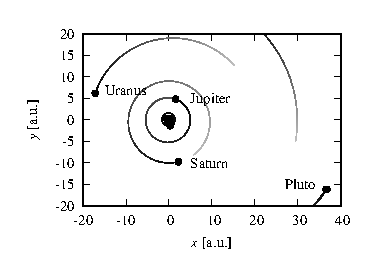
\includegraphics[width = 0.53\textwidth]{figures/gravity.eps}
  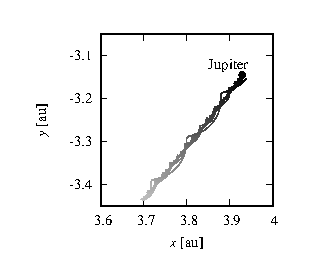
\includegraphics[width = 0.44\textwidth]{figures/Jupiter.eps}
  \end{center}
  \caption{\label{gravity}Motion of objects in the solar system for $10^4$ days 
           starting on the 10th of March 2021, when the code was run. In a 
           close-up of part of the trajectory for Jupiter (\textit{right}), you 
           can also see the trajectories of some of its moons.}
\end{figure}


